\documentclass[a4paper, 12pt, english]{article}

% \usepackage[portuges]{babel}
\usepackage[utf8]{inputenc}
\usepackage{amsmath,amssymb}
\usepackage{graphicx}
\usepackage{subfig}
\usepackage[colorinlistoftodos]{todonotes}

\usepackage{indentfirst}
\usepackage{verbatim}
\usepackage{textcomp}
\usepackage{gensymb}

\usepackage{relsize}

\usepackage{lipsum}% http://ctan.org/pkg/lipsum
\usepackage{xcolor}% http://ctan.org/pkg/xcolor
\usepackage{xparse}% http://ctan.org/pkg/xparse
\NewDocumentCommand{\myrule}{O{1pt} O{2pt} O{black}}{%
  \par\nobreak % don't break a page here
  \kern\the\prevdepth % don't take into account the depth of the preceding line
  \kern#2 % space before the rule
  {\color{#3}\hrule height #1 width\hsize} % the rule
  \kern#2 % space after the rule
  \nointerlineskip % no additional space after the rule
}
\usepackage[section]{placeins}

\usepackage{booktabs}
\usepackage{colortbl}%
   \newcommand{\myrowcolour}{\rowcolor[gray]{0.925}}
   
\usepackage[obeyspaces]{url}
\usepackage{etoolbox}
\usepackage[colorlinks,citecolor=black,urlcolor=blue,bookmarks=false,hypertexnames=true]{hyperref} 

\usepackage{geometry}
\geometry{
	paper=a4paper, % Change to letterpaper for US letter
	inner=3cm, % Inner margin
	outer=3cm, % Outer margin
	bindingoffset=.5cm, % Binding offset
	top=2cm, % Top margin
	bottom=2cm, % Bottom margin
	%showframe, % Uncomment to show how the type block is set on the page
}

\usepackage{amsmath,amsfonts}

\usepackage{listings}


% MATLAB code formatting
\lstdefinestyle{matlab}{
    language=Matlab,
    basicstyle=\scriptsize\ttfamily,
    keywordstyle=\color{blue},
    commentstyle=\color{green!40!black},
    stringstyle=\color{red},
    showstringspaces=false,
    numbers=left,
    numberstyle=\tiny,
    numbersep=5pt,
    tabsize=2,
    breaklines=true,
    breakatwhitespace=true
}
% MATLAB command window formatting
\lstdefinestyle{commandstyle}{
    basicstyle=\scriptsize\ttfamily,
    numbers=none,
    showstringspaces=false,
    breaklines=true,
    frame=single,
    frameround=fttt,
    backgroundcolor=\color{gray!10},
    xleftmargin=0.5cm,
    xrightmargin=0.5cm
}
\usepackage{multicol,caption}
\newenvironment{Figure}
  {\par\medskip\noindent\minipage{\linewidth}}
  {\endminipage\par\medskip}
\usepackage{array}

\newcommand{\highlight}[1]{\textcolor{blue}{\texttt{#1}}}

\graphicspath{{images/}}

%*******************************************************************************%
%************************************START**************************************%
%*******************************************************************************%
\begin{document}

%************************************TITLE PAGE**************************************%
\begin{titlepage}
\begin{center}
\textbf{\LARGE Alexandria University}\\[0.5cm] 
\textbf{\large FACULTY OF ENGINEERING}\\[0.2cm]
\vspace{20pt}

\includegraphics{logo.png}\\[1cm]
\par
\vspace{20pt}
\textbf{\Large EEC382 Introduction to Digital Communications}\\
\vspace{15pt}
\myrule[1pt][7pt]
\textbf{\LARGE  LABORATORY REPORT 1}\\
\vspace{15pt}
\textbf{\large Introduction to probability of error calculation}\\
\myrule[1pt][7pt]
\vspace{25pt}
\textbf{\large \hspace{50pt}Student Name \hspace{60pt} Student ID}\\
Ahmed Osama Mohamed Afifi \hspace{60pt} 20010038 \\

\vspace{45pt}
%\textbf {\large TA in charge:}\\[0.2cm]
%\Large {Hossam Hassan}\\[0.1cm]
\end{center}

\par
\vfill
\begin{center}
\textbf{Submission Date : 26/02/2024}\\
\end{center}

\end{titlepage}

%************************************TABLE OF CONTENTS**************************************%

%  %Sumário
%  \newpage
%  \tableofcontents
%  \thispagestyle{empty}
%  %End Sumário

%********************************%
%***********SECTION 1************%
%********************************%
\newpage
\section{Introduction}
In the realm of wireless communication systems, where signals traverse through dynamic and often unpredictable environments, understanding and quantifying the probability of error is crucial. The Probability of Error Calculation, typically expressed as Bit Error Rate (BER), serves as a fundamental metric in assessing the performance and reliability of wireless communication systems.
\newline

In this laboratory experiment, we employed Monte Carlo simulation as a systematic approach to evaluating the Bit Error Rate in wireless communication systems. The objectives of this experiment remain twofold: first, to investigate the systematic procedure of evaluating the BER in communication systems, and second, to investigate the performance of digital communication system.
\newline

Monte Carlo simulation provides a powerful tool for probabilistic analysis by employing random sampling techniques to model complex systems. By simulating numerous independent trials, we can approximate the behavior of the system and estimate the probability of error with statistical confidence. This approach allows us to explore a wide range of scenarios, including different channel models, modulation schemes, and system configurations, providing valuable insights into the system's performance.
\newline


%********************************%
%***********SECTION 2************%
%********************************%
\newpage
\section{MATLAB code}
\begin{lstlisting}[style=matlab]
% Simulation parameters
NBITS = 1e6;                                % Number of bits/SNR
SNRRANGE = -20 : 2 : 20;                    % Signal to noise ratio range in dB

itterations = 100;                          % Number of itterations for Monte-Carlo simulation
berAvg = 0;                                 % BER average for Monte-Carlo simulation
berVect = zeros(size(SNRRANGE));            % BER results for each SNR

for i = 1 : length(SNRRANGE)
    snrdb  = SNRRANGE(i);
    % Generate random binary data vector
    signal = randi([0 1], 1, NBITS);
    for j = 1 : itterations
        % Apply noise to bits (Hint: you must calculate the signal power in
        % this case because it is not unity)
        signalPWR = mean(signal .^ 2);       % Signal power
        snr = 10 ^ (snrdb / 10);             % SNR
        noisePWR = sqrt(signalPWR / snr);    % Noise power
        noise = noisePWR * randn(1, NBITS);  % Noise vector
        rx_sequence = signal + noise;        % Apply noise to signal
        
        % Decide whether the Rx_sequence is '1' or '0' by comparing the
        % samples (Hint: try to use relational operators and indexing to
        % make the code more efficient)
        signalimg = (rx_sequence > 0.5);
        
        % Compare the original bits with the detected bits and calculate
        % number of errors
        nerrors = sum(signal ~= signalimg);
        ber = nerrors / NBITS;              % BER
        berAvg = berAvg + ber;              % BER accumulator for Monte-Carlo simulation
    end
    berAvg = berAvg / itterations;          % BER average due to Monte-Carlo simulation
    berVect(i) = berAvg;
    berAvg = 0;
end

% Plot the BER curve against SNR (use semilogy)
figure();
title('BER against SNR');
semilogy(SNRRANGE, berVect, '-o');
xlabel('SNR (dB)');
ylabel('Bit Error Rate (BER)');
grid on;
saveas(gcf,'images\BER_against_SNR.png')
fprintf('SNR (dB)	|   BER\n');
fprintf('%6.2f      |   %.8f\n', [SNRRANGE; berVect]);
\end{lstlisting}

\newpage
%********************************%
%***********SECTION 3************%
%********************************%
\section{Results}
\begin{multicols}{2}
\begin{tabular}{>{\raggedright}p{\linewidth} >{\raggedleft}p{0.4\linewidth}}
\begin{Figure}
 \centering
 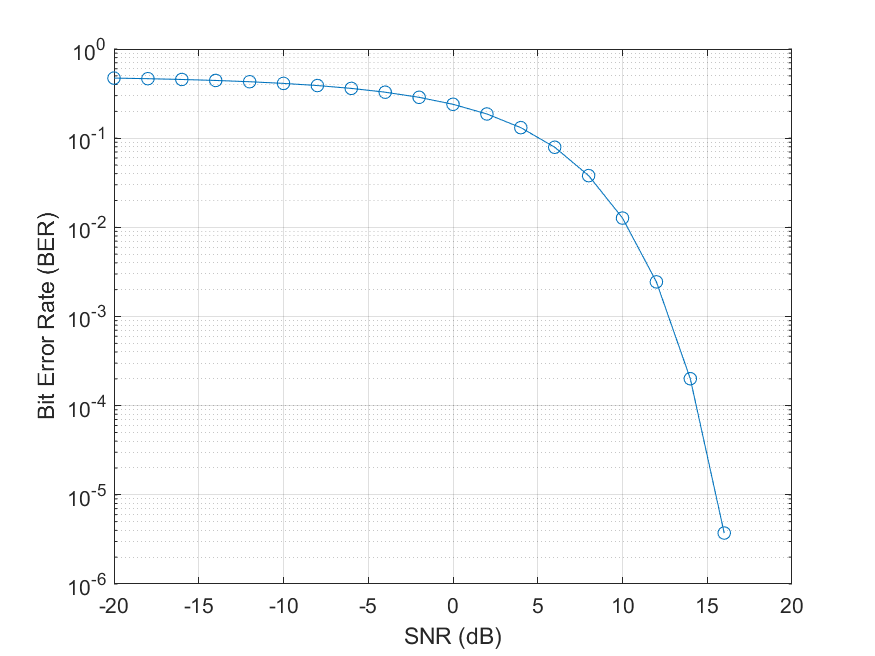
\includegraphics[width=1.2\linewidth, scale=2]{images/BER_against_SNR.png}
 \captionof{figure}{BER against SNR (dB)}
\end{Figure} & \begin{lstlisting}[style=commandstyle, linewidth=170pt]
SNR (dB)    |   BER
-20.00      |   0.47188515
-18.00      |   0.46455504
-16.00      |   0.45532851
-14.00      |   0.44390461
-12.00      |   0.42947836
-10.00      |   0.41150356
 -8.00      |   0.38914331
 -6.00      |   0.36161679
 -4.00      |   0.32780448
 -2.00      |   0.28715680
  0.00      |   0.23977307
  2.00      |   0.18674363
  4.00      |   0.13123180
  6.00      |   0.07910270
  8.00      |   0.03801185
 10.00      |   0.01270070
 12.00      |   0.00244477
 14.00      |   0.00020054
 16.00      |   0.00000373
 18.00      |   0.00000000
 20.00      |   0.00000000
\end{lstlisting} 
\end{tabular}
\end{multicols}

%\begin{figure}
%    \centering
%    \begin{minipage}{0.5\textwidth}
%        \centering
%        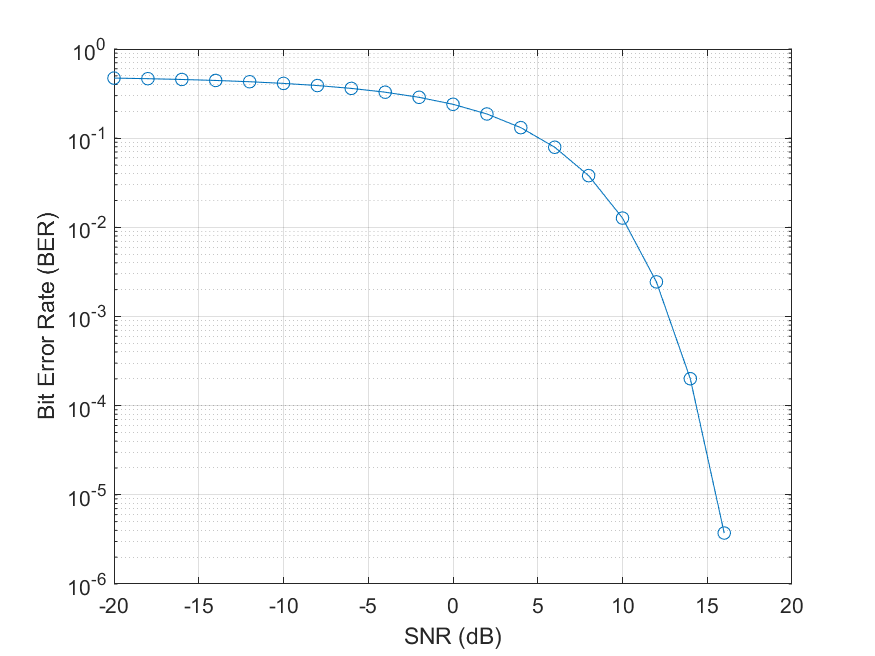
\includegraphics[width=1.2\textwidth]{images/BER_against_SNR.png} % first figure itself
%        \caption{BER against SNR (dB)}
%    \end{minipage}\hfill
%    \begin{minipage}{0.40\textwidth}
%        \centering
%        \begin{lstlisting}[style=commandstyle]
%SNR (dB)    |   BER
%-20.00      |   0.47188515
%-18.00      |   0.46455504
%-16.00      |   0.45532851
%-14.00      |   0.44390461
%-12.00      |   0.42947836
%-10.00      |   0.41150356
% -8.00      |   0.38914331
% -6.00      |   0.36161679
% -4.00      |   0.32780448
% -2.00      |   0.28715680
%  0.00      |   0.23977307
%  2.00      |   0.18674363
%  4.00      |   0.13123180
%  6.00      |   0.07910270
%  8.00      |   0.03801185
% 10.00      |   0.01270070
% 12.00      |   0.00244477
% 14.00      |   0.00020054
% 16.00      |   0.00000373
% 18.00      |   0.00000000
% 20.00      |   0.00000000
%\end{lstlisting}
%    \end{minipage}
%\end{figure}

%********************************%
%***********SECTION 4************%
%********************************%

\section{Calculation of transmitted signal power}
\begin{lstlisting}[style=matlab]
        signalPWR = mean(signal .^ 2);       % Signal power
        snr = 10 ^ (snrdb / 10);             % SNR
        noisePWR = sqrt(signalPWR / snr);    % Noise power
        noise = noisePWR * randn(1, NBITS);  % Noise vector
        rx_sequence = signal + noise;        % Apply noise to signal
\end{lstlisting}
In this code segment, the signal power is computed. The power of a random signal can be determined by computing the mean square over time. \[ \lim_{T\to\infty} \frac{1}{T}\int_{-\frac{T}{2}}^{\frac{T}{2}}{x^2(t,\eta)} \,dx \]
 Hence, we utilize the MATLAB function \highlight{mean} by passing the squared signal to it.


%********************************%
%***********SECTION 5************%
%********************************%
\null\newpage
\section{AWGN channel modelling}

To represent AWGN with its baseband equivalent, we generate a Gaussian distributed signal with a total power equal to the signal power divided by SNR. To simplify, we normalize the signal to unity. Thus, the following equation can be employed: 
\[\text{noise} = \frac{1}{\sqrt{\text{SNR}}} \times \text{randn}\]
Dividing by the square root of SNR (Signal-to-Noise Ratio) is done to scale the noise appropriately relative to the signal power. In communication systems, SNR represents the ratio of signal power to noise power. By dividing by the square root of SNR, we effectively adjust the amplitude of the noise to match the desired SNR level. This ensures that the overall power of the generated noise aligns with the specified SNR, thus accurately modeling the noise level relative to the signal.

\section{SNR and BER relationship}
The point at which the Bit Error Rate (BER) approaches zero depends on several factors such as the modulation scheme, coding techniques, and characteristics of the communication channel. In digital communication systems, an important benchmark is the Shannon Limit, which sets a theoretical upper bound on achievable data rates given a specific Signal-to-Noise Ratio (SNR) and bandwidth. Approaching this limit typically results in very low BER values.

In our specific example, the BER tends towards zero when the SNR reaches 16 dB. This suggests that, at this level of SNR, the system is operating close to its theoretical maximum capacity as defined by the Shannon Limit, resulting in minimal errors in the transmitted data.

\patchcmd{\thebibliography}{\section*}{\section}{}{}

\end{document}